\chapter{Spotfish: A modular framework for decoding spatial imaging data}\label{chap:chapter 3}


\section{Background}

Image-based spatial transcriptomics is a rapidly evolving field that seeks to map the spatial distribution of RNA molecules in situ. These technologies have enabled researchers to study the spatial organization of cells and tissues at unprecedented resolution, with the potential to uncover novel biological insights.The field has seen a surge in interest in recent years, with the development of several novel technologies, including MERFISH\cite{chenSpatiallyResolvedHighly2015}, seqFISH\cite{shahSeqFISHAccuratelyDetects2017}, STARmap\cite{wangThreedimensionalIntacttissueSequencing2018}, ISS\cite{keSituSequencingRNA2013}, and Slide-seq\cite{rodriquesSlideseqScalableTechnology2019}. Despite their varied underlying technologies, they consistently share the same backbone with a unified objective: reporting the location and identity of individual RNA molecules. A significant challenge in this domain is the difficulty in validating the quality of image analysis outputs. This issue is confounded by the lack of standardized data quality metrics accepted by researchers. While existing pipeline development tools for spatial transcriptomics image analysis are functional, they often suffer from limited scalability, a lack of interoperability with newer methodologies, and restricted portability across different computing environments. Recognizing these limitations, there emerges a clear need for an unbiased framework to build spatial transcriptomics pipelines. 

To address these challenges, I developed spotfish, a modular pipeline building framework that abstracts the series of tasks for processing spatial transcriptomics data by standardizing inputs and outputs between workflow tasks. This allows swapping in new tools as new alternatives are published frequently, by wrapping the chosen tool for compatible data formats. It also encourages reporting quality metrics for diagnosing data quality and evaluating the performance of chosen tool/parameter combinations. The framework is built using Nextflow, a robust workflow language specifically built for and heavily adopted by bioinformatics researchers\cite{ditommasoNextflowEnablesReproducible2017}. Nextflow also abstracts how the pipelines are executed on different computing environments, e.g. locally, on compute clusters, or various cloud services, meaning spotfish is inherently usable for researchers regardless of computational environment. In contrast to starfish's approach to programmatic Python-based pipeline construction, spotfish modules are programming language agnostic through the use of containerization for each step of the process. Additionally, the pipeline prioritizes usage of open file formats supported by the Open Microscopy Environment\cite{goldbergOpenMicroscopyEnvironment2005} (OME) to ensure transparency and compatibility with the rich ecosystem of bio-imaging analysis tools. Spotfish is guided by FAIR principles\cite{wilkinsonFAIRGuidingPrinciples2016} and utilize modern open-source standards, ensuring accessibility for a broad spectrum of users, from researchers and core facilities to technologists.

\section{Properties of multiplexed transcriptomics imaging data}

The raw data consists of a large mosaic of microscopy images. To resolve individual fluorescent molecules, images are taken at roughly to 10-100 times magnification. A single image, or field of view, contains roughly 1-100 cells depending on the magnification and cell type. The same field of view is then imaged multiple times, in which the spectrum of light is limited to specific frequency bands at each iteration. This allows us to assign a unique combination of fluorescent probes that emit light at unique frequency bands to each target. The focal plane is much narrower than the height of cells as a consequence of the high magnification, which requires imaging the same field of view multiple times at different z-planes to maximize the volume interrogated. This process is usually repeated for a grid of positions to capture a larger cumulative area of the sample, which can produce upwards of a terabyte of data per experiment. The challenge arises due to the multi-dimensional nature of these measurements, across spatial dimensions x, y and z, channels (multiple laser wavelengths), and rounds (repeated imaging with different combinations of probes).

\section{Framework Design}

Imaging-based acquisition of spatial transcriptomics data requires coordinating a series of tasks, including image stitching, registration, background correction, spot detection, and finally barcode decoding to produce labeled molecular coordinates corresponding to a predesigned set of gene targets. Every task can be accomplished with existing tools, but it remains difficult to perform an end-to-end analysis outside of tailored pipelines without significant data wrangling. Even though many studies utilize commercial platforms for spatial transcriptomics, only processed data is usually available to the customer. Their analysis pipelines remains proprietary and blackbox, forcing users to rely on arbitrarily defined quality metrics. In contrast, starfish is a open-source unified pipeline framework implemented in Python, abstracting processing steps using a object-oriented programming design\cite{othersStarfishOpenSource}. It is extremely flexible and has accommodated data processing for 7 different technologies. However, the API's steep learning curve, many parameters, and lack of maintenance makes it difficult to build pipelines and integrate cutting-edge tools without significant refactoring of the tool or starfish itself. There has only been one prominent third-party contribution by a recent development that integrated their novel barcode decoding algorithm, CheckAll\cite{cisarUnifiedPipelineFISH2023}.

Spotfish abstracts pipelines into two subworkflows: image registration and spot analysis. Image registration is a common image processing step not unique to spatial transcriptomics and is usually required for acquisitions across multiple fields of view. By decoupling this step, it is convenient to adapt tools outside of the immediate domain. The spot analysis subworkflow encompasses two tasks, spot detection and barcode decoding to produce molecular coordinate tables with target i.e. gene annotations. This can then be combined with cell and nuclear segmentation data for functional analysis in other software, such as Bento\cite{mahBentoToolkitSubcellular2022}, Squidpy\cite{pallaSquidpyScalableFramework2021} and Scanpy\cite{wolfSCANPYLargescaleSinglecell2018}.

\begin{figure}[h]
    \centering
    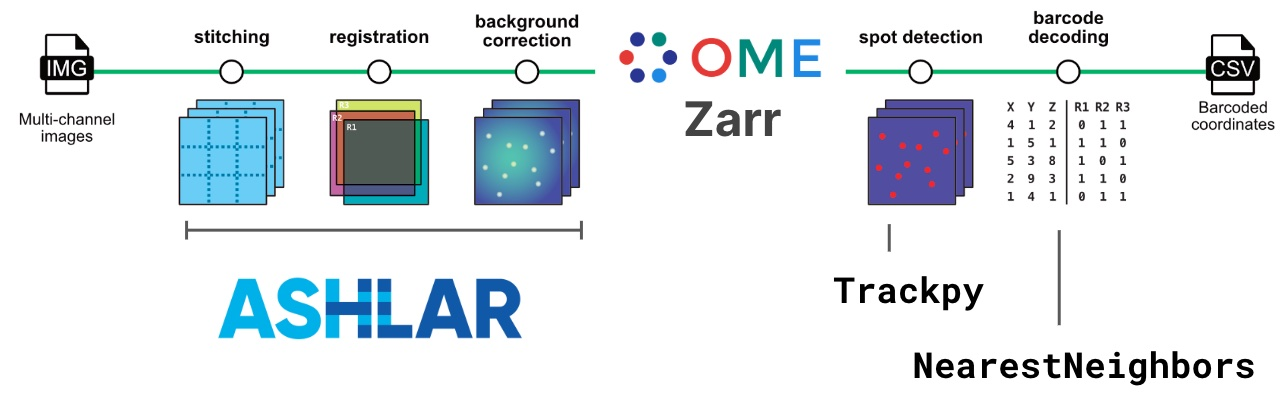
\includegraphics[width=\textwidth]{3_figures-and-files/image processing workflow.jpg}
    \caption[Spotfish workflow]{\textbf{Spotfish workflow} Overview of the analysis tasks in the spotfish workflow from left to right. Image registration encompasses stitching, registration and background correction (as needed). Intermediate output format of OME-ZARR. Spot analysis encompasses spot detection and barcode decoding outputing coordinate tables with annotations. Tools used to implement each subworkflow indicated below.}\label{fig:spotfish workflow}
\end{figure}


\section{Case Study: 69-bit MERFISH of U2-OS Cells}

To demonstrate the utility of spotfish, I applied it to previously published 69-bit MERFISH dataset of U2-OS cells designed to target 10,000 genes with a minimum hamming distance 4 (HD4) encoding scheme\cite{xiaSpatialTranscriptomeProfiling2019}. Because the experiment had a total of 72 rounds of imaging, it was suitable for testing the scalability of the the spotfish framework. Commercial platforms reportedly use 16 rounds (CosMx\cite{heHighplexMultiomicAnalysis2021}) and 15 rounds (Xenium\cite{janesickHighResolutionMapping2022}) to decode 980 and 313 targets respectively. This meant the 10k MERFISH dataset uses roughly 4.5 times more imaging rounds than the current largest commercial platforms. The specific tools implemented in the pipeline were chosen based on their performance on the 10k MERFISH dataset. The image registration step was performed using Ashlar\cite{muhlichStitchingRegisteringHighly2022}, a software package originally designed for stitching and aligning multiplexed immunofluorescent samples acquired via cyclical imaging and tile-scanning. The spot detection step was performed using trackpy\cite{SoftmatterTrackpyV0}, a Python library for particle tracking in 2D and 3D. The barcode decoding step was performed using the nearest neighbor approach implemented in the scikit-learn analysis package\cite{pedregosaScikitlearnMachineLearning2011}.

Spotfish allowed parallelization of the image registration step across all 69 rounds with Ashlar. This step was ultimately limited by memory not computing speed, using 30 GB to stitch each round in 16 cpu hours. The output of the image registration step was a 1.5 TB OME-ZARR file storing a multi-scale representation of the image data registered to the same coordinate system.  By standardizing the output format, this eliminates the need for storing additional metadata defining tile positions and channel orders. The spot detection step was performed using trackpy, which was able to detect 477 million spot coordinates in 3 dimensions. The barcode decoding step was performed using the nearest neighbor approach implemented in the scikit-learn analysis package.  Without spotfish, the total compute time is estimated to be 1248 hours whereas parallelization reduced runtime over 26-fold, to 39 hours with 32 parallel processes for spot detection and 8 parallel processes for spot calling. The output was then visualized using Napari\cite{NapariMultidimensionalImage} to assess the quality of the data interactively.

\section{Conclusion}

All together, I demonstrate spotfish's flexibility in integrating heterogeneous set of tools to build a scalable image analysis pipeline for spatial transcriptomics. By adhering to open file formats and containerization, spotfish addresses existing technologies and is well positioned to adapt to future advancements for image registration, spot detection and barcode decoding. Future work will focus on creating quality control modules that provide quantitative metrics for assessing the quality of the data at each step of the pipeline. This will allow researchers to identify the optimal tool and parameter combinations for their data. To facilitate open discussion of spotfish's development, I aim to collaborate with the nf-core community, a consortium of bioinformatics researchers that develop and maintain a collection of high quality modular bioinformatics pipelines. This will ensure that spotfish is well maintained and accessible to the community. Finally, I will continue to develop spotfish to support additional spatial transcriptomics technologies, such as seqFISH and STARmap. This will allow researchers to compare the performance of different technologies on the same dataset, and to integrate data from different technologies for meta-analysis.